{\scriptsize%
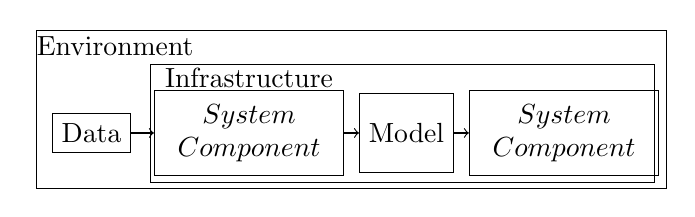
\begin{tikzpicture}
    \node (EnvBox) [rectangle,draw,minimum height =2cm, minimum width=8cm] at (0,0) {};
    \node (Env) at (-3, 0.8) {Environment};

    \node (InfrBox)[rectangle,draw,minimum height =1.5cm, minimum width=6.4cm] at (0.65,-0.18) {};
    \node (Infr) at (-1.3, 0.4) {Infrastructure};

    \node (Data) [rectangle,draw,minimum height =0.5cm, minimum width=0.5cm] at (-3.3,-0.3) {Data};
    \node (Sys1) [rectangle,draw,minimum height =1cm, minimum width=1cm] at (-1.3,-0.3)
        {$\begin{array}{c} \text{System} \\ \text{Component} \end{array}$};
    \node (Model)[rectangle,draw,minimum height =1cm, minimum width=1cm] at (0.7,-0.3) {Model};
    \node (Sys2) [rectangle,draw,minimum height =1cm, minimum width=1cm] at (2.7,-0.3)
        {$\begin{array}{c} \text{System} \\ \text{Component} \end{array}$};

    \draw [->] (Data) -- (Sys1);
    \draw [->] (Sys1) -- (Model);
    \draw [->] (Model) -- (Sys2);

\end{tikzpicture}
}
